\documentclass[10pt, twoside]{book}
    \usepackage[utf8]{inputenc}
    \usepackage[T1]{fontenc}

\usepackage{FileAusiliari/Layout}			% Contiene i pacchetti e le impostazioni per il layout
\usepackage{FileAusiliari/Pacchetti}		% Pacchetti aggiuntivi di vario tipo (senza tikz)
\usepackage{FileAusiliari/TikZ}				% Ambiente tikzpicture
\usepackage{FileAusiliari/Definizioni}		% Definizioni di colori, variabili globali ecc.
\usepackage{FileAusiliari/Environments}		% Impostazioni TOC, bibliografia e indice analitico + environments vari per il contenuto del documento
\usepackage{FileAusiliari/Custom}			% Tutto ciò che è personalizzabile normalmente dall'utente (tranne i colori per collegamenti ipertestuali, citazioni, link, che sono da modificare in Referencing)
\usepackage{FileAusiliari/Referencing}		% Collegamenti ipertestuali e indice analitico
\usepackage{FileAusiliari/Comandi}			% Comandi vari
%%%%%%%%%%%%%%%%%%%%%%%%%%%%
%%%%%%%%%%%%%%%%%%%%%%%%%%%%
\begin{document}
%%%%%%%%%%%%%%%%%%%%%%%%%%%%									 TITOLO
%%%%%%%%%%%%%%%%%%%%%%%%%%%%
\begin{titlepage}
	
    \raggedleft	

    \rule{1pt}{.9\textheight}
	\hspace{0.075\textwidth}
	\parbox[b]{.85\textwidth}{
		{\HUGE\bfseries Titolo
        }\\[2\baselineskip]
		{\Large\textit{Sottotitolo}}\\[47.5\baselineskip]
        {\Large\textsc{autore}}\\[1\baselineskip]
        
	}
\end{titlepage}
%%%%%%%%%%%%%%%%%%%%%%%%%%%%									FRONTMATTER
%%%%%%%%%%%%%%%%%%%%%%%%%%%%
\frontmatter
\pagestyle{fancyfront}
%%%%%								 INDICE
\begingroup
{
	\let\cleardoublepage\relax
	%%%%%		Nome Indice (NASCOSTO E CREATO A PARTE)
	\renewcommand\contentsname{}
	\begin{tikzpicture}[remember picture, overlay]
		\clip (-80,-95) rectangle (40,10);
		\pgftext[x=.8\textwidth, y=0.2cm]{\HUGE\bfseries 
		Indice}						% Titolo indice
		\end{tikzpicture}
	\vspace{-1cm}
	
	\tableofcontents*
	\vspace{.25cm}
}
%%%%%								INTRODUZIONE
		\titleformat{\chapter}
		[hang]
		{\Huge}
		{}
		{0em}
		{}
		[\Large {\begin{tikzpicture} [remember picture, overlay]
		\pgftext[right,x=14.75cm,y=0.2cm]{\HUGE\bfseries 
			Introduzione}
		\end{tikzpicture}}]
%%%%%%%%%%%%%%%%%%%%%%%%%%%%%%%%%%%%%%%%%%%%%%%%%%%%%%%%%%%%%%%%%%%%%%%%%%%%%%%%%
\chapter*{}\normalfont\addcontentsline{toc}{part}{Introduzione}
\lipsum
\endgroup

%%%%%								ERRATA 
\iffalse
		\titleformat{\chapter}
		[hang]
		{\huge}
		{}
		{0em}
		{}
		[\large {\begin{tikzpicture} [remember picture, overlay]
		\pgftext[right,x=14.75cm,y=0.2cm]{\color{black}\Huge\bfseries 
			Errata corrige \& Aggiunte};
		\end{tikzpicture}}]
\chapter*{}\normalfont		\addcontentsline{toc}{part}{Errata corrige \& Aggiunte}
\begin{longtable}{p{2.55cm}p{1.45cm}p{9cm}}
	Data di \newline correzione & Pagina&\\\hline
	24/10/2023	& ?	& ?
\end{longtable}
\fi

%%%%%%%%%%%%%%%%%%%%%%%%%%%%									MAINMATTER
%%%%%%%%%%%%%%%%%%%%%%%%%%%%
\mainmatter

\pagestyle{fancymain}
\titleformat{\chapter}[display]{\bfseries\Large}	{\filleft\MakeUppercase{\chaptertitlename} \HUGE\thechapter}{.5ex}{\titlerule\vspace{.1ex}\filleft}[\vspace{.5ex}]
\titlespacing*{\chapter}{0pt}{0.1\baselineskip}{0.5\baselineskip}

\fancyheadoffset[L]{\dimexpr\oddsidemargin-0in\relax}
\fancyheadoffset[R]{\dimexpr\oddsidemargin-0in\relax}

\normalfont
\normalsize


\newgeometry{top=35mm, bottom=35mm, left=15mm, right=15mm, headheight=0pt, headsep=0pt, marginparsep=0pt, marginparwidth=0pt, footskip=0pt, footnotesep=0pt}
\part*{\HUGE Parte 1}\label{Parte1}
\restoregeometry

%%%%%								CAPITOLI
\chapter{Environments}
\section{Teoremi, dimostrazioni, proposizioni, lemmi, corollari}
	\begin{verbatim}
		\begin{The}		\lipsum[1]		\end{The}
	\end{verbatim}
\begin{The}		\lipsum[1]		\end{The}

	\begin{verbatim}
		\begin{Proof}		\lipsum[1]		\end{Proof}
	\end{verbatim}
\begin{Proof}	\lipsum[2]		\end{Proof}

\begin{verbatim}
	\begin{Pro}		\lipsum[1]		\end{Pro}
\end{verbatim}
\begin{Pro}		\lipsum[3] 		\end{Pro}

\begin{verbatim}
	\begin{Le}		\lipsum[1]		\end{Le}
\end{verbatim}
\begin{Le}			\lipsum[5]		\end{Le}

\begin{verbatim}
	\begin{Co}		\lipsum[1]		\end{Co}
\end{verbatim}
\begin{Co}		\lipsum[6]		\end{Co}
%%%%%%%%%%%%%%%%%%%%%%%%%%%%%%%%%%%
\section{Definizioni, esempi, osservazioni}
\begin{verbatim}
	\begin{De}		\lipsum[1]		\end{De}
\end{verbatim}
\begin{De}		\lipsum[7]		\end{De}

\begin{verbatim}
	\begin{Exa}		\lipsum[1]		\end{Exa}
\end{verbatim}\begin{Exa}\lipsum[8] \end{Exa}

\begin{verbatim}
	\begin{Oss}		\lipsum[1]		\end{Oss}
\end{verbatim}
\begin{Oss}\lipsum \end{Oss}
%%%%%%%%%%%%%%%%%%%%%%%%%%%%%%%%%%%
\section{Description, itemize, enumerate}
\paragraph*{} \underline{Description}
\begin{verbatim}
	\begin{description}		\item[Oggetto 1] Prova \item[Oggetto 2] Prova		\end{description}
\end{verbatim}
\begin{description}
	\item[Oggetto 1] Prova 
	\item[Oggetto 2] Prova 
\end{description}

\begin{verbatim}
	\begin{itemize}		\item Prova \item Prova \item Prova		\end{itemize}
\end{verbatim}
\paragraph*{} \underline{Itemize}
\begin{itemize}
	\item Prova 
	\item Prova
	\item \lipsum[9]
\end{itemize}

\begin{verbatim}
	\begin{enumerate}		\item Prova \item Prova		\end{enumerate}
\end{verbatim}
\paragraph*{} \underline{Enumerate}
\begin{enumerate}
	\item Prova
	\item Prova
\end{enumerate}
%%%%%%%%%%%%%%%%%%%%%%%%%%%%%%%%%%%
\section{Note a margine}
	\lipsum[1]
	\note{Nota a margine: può essere utile come segnaposto per definizioni, teoremi... Si usa col comando \text{$\setminus$note\{\#1\}}}
	\lipsum[1]
	\lipsum[1]
		\expl{Ho impostato una versione con un colore diverso per spiegare passaggi nelle dimostrazioni. Si usa col comando \text{$\setminus$expl\{\#1\}}}
	\lipsum[1]
%%%%%%%%%%%%%%%%%%%%%%%%%%%%%%%%%%%
\section{Collegamenti ipertestuali, citazioni, indici, url}
	\paragraph*{} Un collegamento ipertestuale si realizza con
\begin{verbatim}\label{Label}\end{verbatim}		
e si richiama con
 \begin{verbatim}\ref{LabelTesto}\end{verbatim}
 Risultato: \label{LabelTesto}\ref{LabelTesto}

\paragraph*{} Una citazione a un libro in bibliografia si realizza con
\begin{verbatim}\cite{LabelLibro}\end{verbatim}
	Risultato: \cite{Label}

\paragraph*{} Si inserisce un nuovo elemento nell'indice analitico con i comandi
\begin{verbatim}\index{Index}\end{verbatim}
\begin{verbatim}\index{Index!SecondaVoce}\end{verbatim}
Per il risultato di questi comandi vedere l'indice analitico a fine documento. \index{Index}\index{Index!SecondaVoce}
\paragraph*{} Per mettere un link si può usare
\begin{verbatim}\url{https://poisson.phc.dm.unipi.it/~puddu}\end{verbatim}
Risultato: \url{https://poisson.phc.dm.unipi.it/~puddu}
%
\chapter{Nuovi comandi introdotti in 'Custom.sty'}
\Minipage{.45}{\begin{longtable}{r|r|r}
Mathbb ($\setminus$A)& Mathcal ($\setminus$AA) & Mathscr ($\setminus$AAA)\\\hline
$\A$ & $\AA$ & $\AAA$\\[0.1cm]
$\B$ & $\BB$ & $\BBB$\\[0.1cm]
$\C$ & $\CC$ & $\CCC$\\[0.1cm]
$\D$ & $\DD$ & $\DDD$\\[0.1cm]
$\E$ & $\EE$ & $\EEE$\\[0.1cm]
$\F$ & $\FF$ & $\FFF$\\[0.1cm]
$\G$ & $\GG$ & $\GGG$\\[0.1cm]
$\H$ & $\HH$ & $\HHH$\\[0.1cm]
$\I$ & $\II$ & $\III$\\[0.1cm]
$\J$ & $\JJ$ & $\JJJ$\\[0.1cm]
$\K$ & $\KK$ & $\KKK$\\[0.1cm]
$\L$ & $\LL$ & $\LLL$\\[0.1cm]
$\M$ & $\MM$ & $\MMM$\\[0.1cm]
$\N$ & $\NN$ & $\NNN$\\[0.1cm]
$\O$ & $\OO$ & $\OOO$\\[0.1cm]
$\P$ & $\PP$ & $\PPP$\\[0.1cm]
$\Q$ & $\QQ$ & $\QQQ$\\[0.1cm]
$\R$ & $\RR$ & $\RRR$\\[0.1cm]
$\S$ & $\SS$ & $\SSS$\\[0.1cm]
$\T$ & $\TT$ & $\TTT$\\[0.1cm]
$\U$ & $\UU$ & $\UUU$\\[0.1cm]
$\V$ & $\VV$ & $\VVV$\\[0.1cm]
$\W$ & $\WW$ & $\WWW$\\[0.1cm]
$\X$ & $\XX$ & $\XXX$\\[0.1cm]
$\Y$ & $\YY$ & $\YYY$\\[0.1cm]
$\Z$ & $\ZZ$ & $\ZZZ$\\[0.1cm]
\end{longtable}
}{.35}{
\begin{longtable}{rl}
& \bf Simboli\\\hline
\text{$\setminus$d}& $\d$ \\[0.1cm]
\text{$\setminus$e}& $\e$ \\[0.1cm]
\text{$\setminus$exp}& $\exp$ \\[0.1cm]
\text{$\setminus$f}& $\f$ \\[0.1cm]
\text{$\setminus$g}& $\g$ \\[0.1cm]
\text{$\setminus$i}& $\i$ \\[0.1cm]
\text{$\setminus$Id\{A\}}& $\Id{A}$ \\[0.1cm]
\text{$\setminus$j}& $\j$ \\[0.1cm]
\text{$\setminus$l}& $\l$ \\[0.1cm]
\text{$\setminus$sbullet}& $\sbullet$ \\[0.1cm]
\text{$\setminus$v}& $\v$ \\[0.1cm]
\text{$\setminus$Zero}& $\Zero$ \\[0.1cm]
\end{longtable}
\begin{longtable}{rl}
& \bf Operatori\\\hline
\text{$\setminus$*}& $\*$ \\[0.1cm]
\text{$\setminus$CF\{A\}\{B\}}& $\CF{A}{B}$ \\[0.1cm]
\text{$\setminus$codim\{A\}\{B\}}& $\codim{A}{B}$ \\[0.1cm]
\text{$\setminus$Dif\{A\}\{B\}}& $\Dif{A}{B}$ \\[0.1cm]
\text{$\setminus$Diff\{A\}\{B\}}& $\Diff{A}{B}$ \\[0.1cm]
\text{$\setminus$Floor\{A\}}& $\Floor{A}$ \\[0.1cm]
\text{$\setminus$Imm\{A\}}& $\Imm{A}$ \\[0.1cm]
\text{$\setminus$Leg\{A\}\{B\}}& $\Leg{A}{B}$ \\[0.1cm]
\text{$\setminus$nobarfrac\{A\}\{B\}}& $\nobarfrac{A}{B}$ \\[0.1cm]
\text{$\setminus$Norma\{A\}}& $\Norma{A}$ \\[0.1cm]
\text{$\setminus$Lie\{A\}\{B\}}& $\Lie{A}{B}$ \\[0.1cm]
\text{$\setminus$PS\{A\}\{B\}}& $\PS{A}{B}$ \\[0.1cm]
\text{$\setminus$Rad\{A\}}& $\Rad{A}$ \\[0.1cm]
\text{$\setminus$Re\{A\}}& $\Re{A}$ \\[0.1cm]
\text{$\setminus$Res\{A\}\{B\}}& $\Res{A}{B}$ \\[0.1cm]
\text{$\setminus$Stirling\{A\}\{B\}}& $\Stirling{A}{B}$ \\[0.1cm]
\text{$\setminus$Val\{A\}\{B\}}& $\Val{A}{B}$ \\[0.1cm]
\end{longtable}
}
\newpage
\begin{longtable}{rl}
&\bf Insiemi e gruppi\\\hline
\text{$\setminus$Ann\{A\}}& $\Ann{A}$ \\[0.1cm]
\text{$\setminus$Aut\{A\}}& $\Aut{A}$ \\[0.1cm]
\text{$\setminus$Fix\{A\}}&$\Fix{A}$ \\[0.1cm]
\text{$\setminus$GAut\{A\}}& $\GAut{A}$ \\[0.1cm]
\text{$\setminus$GL\{A\}\{B\}}& $\GL{A}{B}$ \\[0.1cm]
\text{$\setminus$GLE\{A\}}& $\GLE{A}$ \\[0.1cm]
\text{$\setminus$Hom\{A\}\{B\}\{C\}}& $\Hom{A}{B}{C}$ \\[0.1cm]
\text{$\setminus$Im\{A\}}& $\Im{A}$ \\[0.1cm]
\text{$\setminus$Ker\{A\}}& $\Ker{A}$ \\[0.1cm]
\text{$\setminus$OM\{A\}\{B\}}& $\OM{A}{B}$ \\[0.1cm]
\text{$\setminus$Seq\{A\}\{B\}\{C\}}& $\Seq{A}{B}{C}$ \\[0.1cm]
\text{$\setminus$Set\{A\}}& $\Set{A}$ \\[0.1cm]
\text{$\setminus$SLM\{A\}\{B\}}& $\SLM{A}{B}$ \\[0.1cm]
\text{$\setminus$SO\{A\}\{B\}}& $\SO{A}{B}$ \\[0.1cm]
\text{$\setminus$Span\{A\}}& $\Span{A}$ \\[0.1cm]
\text{$\setminus$SU\{A\}\{B\}}& $\SU{A}{B}$ \\[0.1cm]
\text{$\setminus$Stab\{A\}\{B\}}& $\Stab{A}{B}$ \\[0.1cm]
\text{$\setminus$TM\{A\}\{B\}}& $\TM{A}{B}$ \\[0.1cm]
\text{$\setminus$Tr\{A\}}& $\Tr{A}$ \\[0.1cm]
\text{$\setminus$UM\{A\}\{B\}}& $\UM{A}{B}$ \\[0.1cm]
\end{longtable}
%%%%%%%%%%%%%%%%%%%%%%%%%%%%%%%%%%%
\section{Ambienti equazione}
\begin{verbatim}
\EqL{Equazione con label}{B}
\end{verbatim}
\EqL{Equazione\ con\ label}{B}

\begin{verbatim}\Eq{A & B\\ C & D}\end{verbatim}
\Eq{A& B\\C&D}
%%%%%%%%%%%%%%%%%%%%%%%%%%%%%%%%%%%
\section{Ambienti funzione}	
\begin{verbatim}
\Map{A}{B}{C}{D}{E}
\end{verbatim}
$$\Map{A}{B}{C}{D}{E}$$

\begin{verbatim}
\NMap{A}{B}{C}{D}
\end{verbatim}
$$\NMap{A}{B}{C}{D}$$
%%%%%%%%%%%%%%%%%%%%%%%%%%%%%%%%%%%
\section{Ambiente introduzione ai capitoli (ad esempio)}
\begin{verbatim}
\begin{TitoloIntro}[colbacktitle=red, width=\textwidth]{Titolo}{Riquadro}\end{TitoloIntro}
\end{verbatim}
\begin{TitoloIntro}[colbacktitle=red, width=\textwidth]{Titolo}{Riquadro}\end{TitoloIntro}

\begin{verbatim}
\begin{RTitoloIntro}[colbacktitle=red]{Titolo}{Riquadro}\end{RTitoloIntro}
\end{verbatim}
\begin{RTitoloIntro}[colbacktitle=red]{Titolo}{Riquadro}\end{RTitoloIntro}
%%%%%%%%%%%%%%%%%%%%%%%%%%%%%%%%%%%
\section{Ambiente minipage}
\begin{verbatim}
\Minipage{0.5}{Pagina a sinistra}{0.5}{Pagina a destra}
\end{verbatim}
\Minipage{0.5}{Pagina a sinistra}{0.5}{Pagina a destra}	
%%%%%%%%%%%%%%%%%%%%%%%%%%%%%%%%%%%
\section{Citazione}
\begin{verbatim}
\Quote{A}{B}{.5}
\end{verbatim}
\Quote{A}{B}{.5}
%%%%%%%%%%%%%%%%%%%%%%%%%%%%%%%%%%%
\section{Pacchetto "polynomial"}
\paragraph*{}Offre un migliore typesetting dei polinomi (si scrivono solo i coefficienti: la variabile e gli esponenti sono gestiti con le opzioni all'inizio del comando e non si devono scrivere in ogni monomio). Una lista esaustiva di comandi disponibili è la seguente:
\begin{center}
\begin{minipage}{.7\textwidth}
\begin{verbatim}
\polynomial{1,1,2,c,0,0,0,0,5}
\end{verbatim}
%Lista dei coefficienti di x^0, x^1,x^2 ecc
\end{minipage}
\begin{minipage}{.2\textwidth}
\Eq{\polynomial{1,1,2,c,0,0,0,0,5}}
\end{minipage}
\begin{minipage}{.7\textwidth}
\begin{verbatim}
\polynomialfrac{1,1,2,c,0,0,0,0,5}{0,1,1,4}
\end{verbatim}
%Funzione razionale: elenca i coefficienti
\end{minipage}
\begin{minipage}{.2\textwidth}
\Eq{\polynomialfrac{1,1,2,c,0,0,0,0,5}{0,1,1,4}}
\end{minipage}
\begin{minipage}{.7\textwidth}
\begin{verbatim}	
\polynomial[falling]{a,b,c,-d,e}
\end{verbatim}
\end{minipage}
\begin{minipage}{.2\textwidth}\vspace{-.1cm}
\Eq{\hspace{-1cm}\polynomial[falling]{a,b,c,-d,e}}
\end{minipage}
\begin{minipage}{.6\textwidth}
\begin{verbatim}
\polynomial[reciprocal]{a,b,c,d,e}
\end{verbatim}
\end{minipage}
\begin{minipage}{.3\textwidth}
\Eq{\polynomial[reciprocal]{a,b,c,d,e}}
\end{minipage}
\begin{minipage}{.7\textwidth}
\begin{verbatim}
\polynomial[var=t]{1,1,2,c,0,0,0,0,5}
\end{verbatim}
\end{minipage}
\begin{minipage}{.2\textwidth}
\Eq{\polynomial[var=t]{1,1,2,c,0,0,0,0,5}}
\end{minipage}
\begin{minipage}{.6\textwidth}
\begin{verbatim}
\polynomial[start=1000]{1,1,2,c,0,0,0,0,5}
\end{verbatim}
\end{minipage}
\begin{minipage}{.35\textwidth}
\Eq{\polynomial[start=1000]{1,1,2,c,0,0,0,0,5}}
\end{minipage}
\begin{minipage}{.7\textwidth}
\begin{verbatim}
\polynomial[step=-5]{1,1,2,c}
\end{verbatim}
\end{minipage}
\begin{minipage}{.2\textwidth}
\Eq{\polynomial[step=-5]{1,1,2,c}}
\end{minipage}
\begin{minipage}{.7\textwidth}
\begin{verbatim}\polynomial[add=\otimes]{1,1,2,c,0,0,0,0,5}
\end{verbatim}
\end{minipage}
\begin{minipage}{.2\textwidth}
\Eq{\polynomial[add=\otimes]{1,1,2,c,0,0,0,0,5}}
\end{minipage}
\begin{minipage}{.7\textwidth}
\begin{verbatim}\polynomial[sub=\times]{1,2,-c,0,0,0,0,-5}
\end{verbatim}
\end{minipage}
\begin{minipage}{.2\textwidth}
\Eq{\polynomial[sub=\times]{1,2,-c,0,0,0,-5}}
\end{minipage}
\end{center}
%%%%%%%%%%%%%%%%%%%%%%%%%%%%%%%%%%%
\section{Pacchetto "accents"}
\paragraph*{} Migliora il typesetting di lettere accentate in ambiente matematico. Ad esempio
\begin{center}
\begin{minipage}{.4\textwidth}
\begin{verbatim}
\undertilde{Prova}
\end{verbatim}
\end{minipage}
\begin{minipage}{.2\textwidth}
\Eq{\undertilde{Prova}}
\end{minipage}
\begin{minipage}{.4\textwidth}
\begin{verbatim}
\underaccent{under}{a}
\end{verbatim}
\end{minipage}
\begin{minipage}{.2\textwidth}
\Eq{\underaccent{under}{a}}
\end{minipage}
\begin{minipage}{.4\textwidth}
\begin{verbatim}
\accentset{over}{a}
\end{verbatim}
\end{minipage}
\begin{minipage}{.2\textwidth}
\Eq{\accentset{over}{a}}
\end{minipage}
\begin{minipage}{.4\textwidth}
\begin{verbatim}
\hat{\accentset{\pi}{a}}
\end{verbatim}
\end{minipage}
\begin{minipage}{.2\textwidth}
\Eq{\hat{\accentset{over}{a}}}
\end{minipage}
\begin{minipage}{.4\textwidth}
\begin{verbatim}
\ring{a}
\end{verbatim}
\end{minipage}
\begin{minipage}{.2\textwidth}
\Eq{\ring{a}}
\end{minipage}
\begin{minipage}{.4\textwidth}
\begin{verbatim}
\overrightarrow{Testo}
\end{verbatim}
\end{minipage}
\begin{minipage}{.2\textwidth}
\Eq{\overrightarrow{Testo}}
\end{minipage}
\begin{minipage}{.4\textwidth}
\begin{verbatim}
 \underrightarrow{Testo}
\end{verbatim}
\end{minipage}
\begin{minipage}{.2\textwidth}
\Eq{ \underrightarrow{Testo}}
\end{minipage}
\begin{minipage}{.4\textwidth}
\begin{verbatim}
\xrightarrow[Sotto]{Sopra}
\end{verbatim}
% da usare al posto di overset quando c'è un commento sopra/sotto una freccia in una equazione
\end{minipage}
\begin{minipage}{.2\textwidth}
\Eq{\xrightarrow[Sotto]{Sopra}}
\end{minipage}
\begin{minipage}{.4\textwidth}
\begin{verbatim}
\overset{Sopra}{Testo}
\end{verbatim}
\end{minipage}
\begin{minipage}{.2\textwidth}
\Eq{\overset{Sopra}{Testo}}
\end{minipage}
\begin{minipage}{.4\textwidth}
\begin{verbatim}
\underset{Sotto}{Testo}
\end{verbatim}
\end{minipage}
\begin{minipage}{.2\textwidth}
\Eq{\underset{Sotto}{Testo}}
\end{minipage}
\begin{minipage}{.4\textwidth}
\begin{verbatim}
$$ \sideset{_a^b}{_c^d}\sum$$
\end{verbatim}
% Per mettere accenti vicino a simboli di sum, prod, bigoplus, bigotimes, ecc.
\end{minipage}
\begin{minipage}{.2\textwidth}
\Eq{\sideset{_a^b}{_c^d}\sum}\vspace{1cm}
\end{minipage}
\end{center}
%%%%%%%%%%%%%%%%%%%%%%%%%%%%%%%%%%%
\section{Typesetting di formule matematiche in \$ \$}
\begin{verbatim}
$\tfrac{Numeratore}{Denominatore}$
\end{verbatim}
Testo $\tfrac{Numeratore}{Denominatore}$ Testo

\begin{verbatim}
$\tbinom{N}{D}$
\end{verbatim}
Testo $\tbinom{N}{D}$ Testo
\chapter{TikZ e plotting}
\section{Boxes}
\begin{verbatim}
\boxed{Prova}
\end{verbatim}
$$\boxed{Prova}$$

\begin{verbatim}
	\RiquadroOmbra{Testo}
\end{verbatim}
\RiquadroOmbra{Testo}

\begin{verbatim}
	\begin{TitoloIntro}[colbacktitle=red]{Titolo}{Testo}\end{TitoloIntro}
\end{verbatim}
\begin{TitoloIntro}[colbacktitle=red, width=\textwidth]{Titolo}{Testo}\end{TitoloIntro}

\begin{verbatim}
	\begin{RTitoloIntro}[colbacktitle=red]{Titolo}{Testo}\end{RTitoloIntro}
\end{verbatim}
\begin{RTitoloIntro}[colbacktitle=red]{Titolo}{Testo}\end{RTitoloIntro}
%%%%%%%%%%%%%%%%%%%%%%%%%%%%%%%%%%%%%%%%%%%%%%%%%%%%%%
\newpage
\section{PGF (per info sul typesetting -> "pgfplots" su ctan.org)}
\paragraph*{} Questa sezione contiene solo alcuni esempi.

\begin{verbatim}
	\begin{figure}[ht]\centering
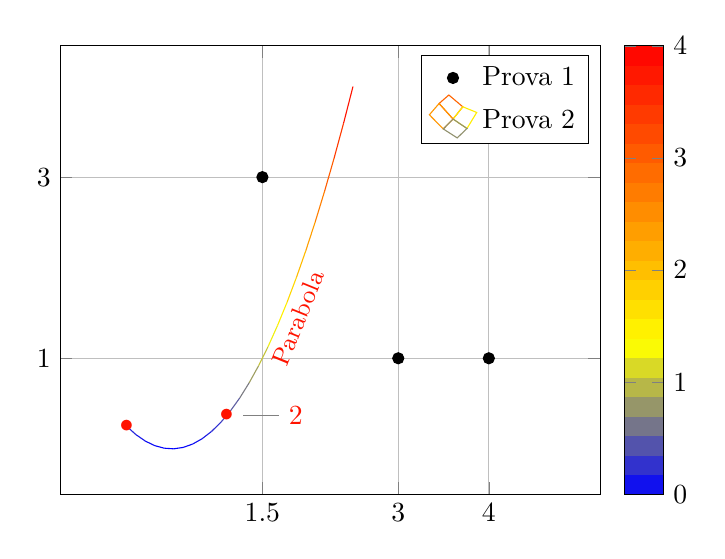
\begin{tikzpicture} \begin{axis}[xmin=-0.5, xmax=5, ymin=-0.5,
	colorbar sampled, colorbar style={samples=24}, 
	axis equal, xtick=data, ytick=data, grid=major]
    \addplot[only marks] coordinates { (4,1) (3,1) (1.5,3) };
   	\addplot[mesh, domain=0:2.5, tick=\empty] {(x-.5)^2}  node [pos=0]  {$\bullet$}      
   	node [pos=0.25, pin=0.4:2 ] {$\bullet$}
   	node [pos=0.5, sloped, xshift=0cm, yshift=-.2cm] {\small Parabola}; 
     \legend{Prova 1, Prova 2};     
\end{axis}	
\end{tikzpicture}\noindent\hspace{2cm}
\caption{}	
\end{verbatim}
\begin{figure}[ht]\centering
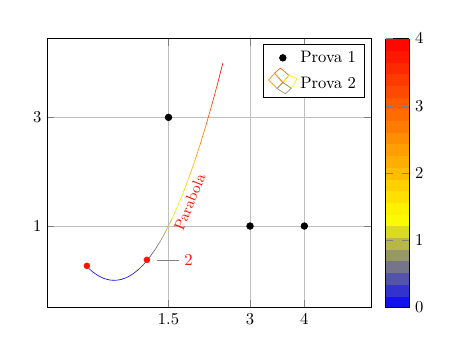
\begin{tikzpicture}[scale=.6] \begin{axis}[
xmin=-0.5, xmax=5, ymin=-0.5, colorbar sampled, colorbar style={samples=24}, axis equal, xtick=data, ytick=data, grid=major]
    \addplot[only marks] coordinates {  (4,1) (3,1) (1.5,3)    };
   	\addplot[mesh, domain=0:2.5, tick=\empty] {(x-.5)^2}  node [pos=0]    {$\bullet$}            node [pos=0.25, pin=0.4:2 ] {$\bullet$}            node [pos=0.5, sloped, xshift=0cm, yshift=-.2cm]  {\small Parabola}    ; 
     \legend{Prova 1, Prova 2};     
\end{axis}	
\end{tikzpicture}\noindent\hspace{2cm}
\caption{Colormap, legenda, punti e grafici di funzione}
\end{figure}

\newpage

\begin{verbatim}
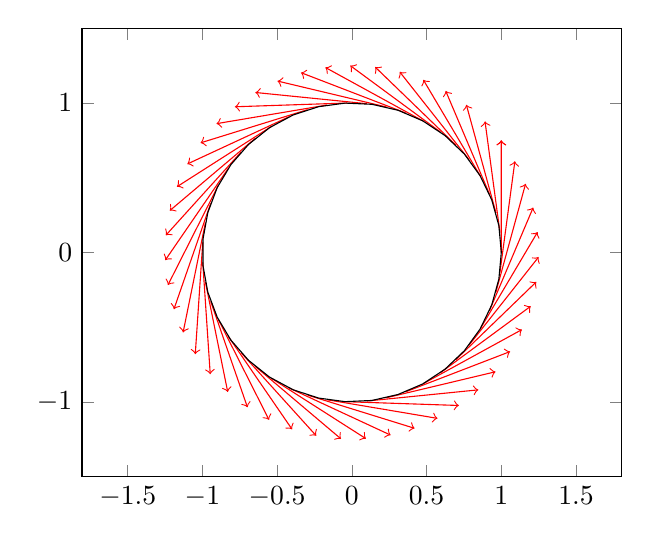
\begin{tikzpicture} \begin{axis}[
    axis equal, xmin=-1.5, xmax=1.5, ymin=-1.5, ymax=1.5]
    \addplot [samples=48, domain=0:2*pi,->,blue, variable=\t,
        quiver={
            u={-sin(deg(t))},
            v={cos(deg(t))},
            scale arrows=0.75,
            colored=red},] ({cos(deg(t))}, {sin(deg(t))});
    \addplot [samples=36, domain=0:2*pi] ( {cos(deg(x))}, {sin(deg(x))} );
\end{axis}
\end{tikzpicture}	
\end{verbatim}
\begin{figure}[ht]\centering
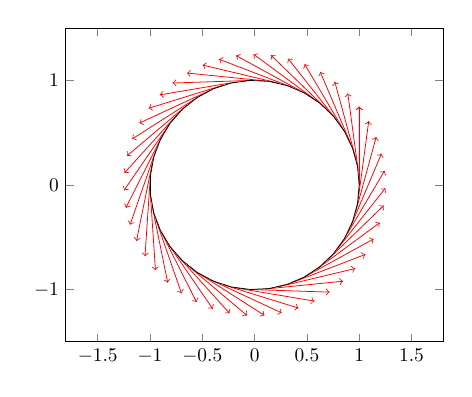
\begin{tikzpicture}[scale=.7] \begin{axis}[
    axis equal, xmin=-1.5, xmax=1.5, ymin=-1.5, ymax=1.5]
    \addplot [samples=48, domain=0:2*pi,->,blue, variable=\t,
        quiver={
            u={-sin(deg(t))},
            v={cos(deg(t))},
            scale arrows=0.75,
            colored=red},] ({cos(deg(t))}, {sin(deg(t))});
    \addplot [samples=36, domain=0:2*pi] ( {cos(deg(x))}, {sin(deg(x))} );
\end{axis}
\end{tikzpicture}
\caption{Parametrizzazioni}
\end{figure}

\newpage

\begin{verbatim}
\begin{figure}[ht]\centering
\begin{tikzpicture}
\begin{axis}[xmin=-5, xmax=5, ymin=-28, axis equal]
\addplot [samples=24, domain=0:2*pi, dashed, data cs=polar,
	top color=Blues-I, bottom color=Blues-B] (deg(x),30);
\addplot [name path=Y, samples=24, domain=0:2*pi, dashed,
    data cs=polar] (deg(x),30);
\addplot [GnBu-M, name path=X, domain=0:360, samples=36,
    smooth, data cs=polar](x, {30-8*sin(3*x)});
\addplot[green] fill between[of=Y and X];
\addplot [samples=36,domain=0:30, dashed,
    data cs=cart] {.025*x^2} node [pos=1] {Nodo};
\addplot [mark=oplus, only marks] coordinates {(0,0)};
\node[pin=120:{Pin nodo}] at (0,0) {};
\end{axis}
\end{tikzpicture}
\end{figure}	
\end{verbatim}
\begin{figure}[ht]\centering
\begin{tikzpicture}[scale=.8]
\begin{axis}[xmin=-5, xmax=5, ymin=-28, axis equal]
\addplot [samples=24, domain=0:2*pi, dashed, data cs=polar, top color=Blues-I, bottom color=Blues-B    ] (deg(x),30);
\addplot [name path=Y, samples=24, domain=0:2*pi, dashed,
    data cs=polar] (deg(x),30);
\addplot [GnBu-M, name path=X, domain=0:360, samples=36,
    smooth, data cs=polar](x, {30-8*sin(3*x)});
\addplot[green] fill between[of=Y and X];
\addplot [samples=36, domain=0:30, dashed,
    data cs=cart] {.025*x^2} node [pos=1] {Nodo};
\addplot [mark=oplus, only marks] coordinates {(0,0)};
\node[pin=120:{Pin nodo}] at (0,0) {};
\end{axis}
\end{tikzpicture}
\caption{Filling, nodi e pin}
\end{figure}

\newpage

\begin{verbatim}
\begin{tikzpicture}[scale=.8]
\begin{axis}[axis equal=false, xmin=-1, xmax=2, ymin=-3.5, ymax=1]
\addplot[red, patch type sampling, patch type= cubic spline, domain=0:2, smooth]{ln(x)};
\draw (0,0) .. controls (1,-1.2) and (1,1) .. (2,1);
   \end{axis}
\end{tikzpicture}	
\end{verbatim}
\begin{figure}[ht]\centering
\begin{tikzpicture}
\begin{axis}[axis equal=false, xmin=-1, xmax=2, ymin=-3.5, ymax=1]
\addplot[red, patch type sampling, patch type= cubic spline, domain=0:2, smooth]{ln(x)};
\draw (0,0) .. controls (1,-1.2) and (1,1) .. (2,1);
   \end{axis}
\end{tikzpicture}
\caption{Interpolazione, pathing}
\end{figure}

\newpage

\begin{verbatim}
\begin{tikzpicture}
\begin{axis}[
    colormap/PuBu,
    samples=12, domain=-5:5, y domain=-4:4,  xmin=-5, xmax=5, ymin=-4, ymax=4]
    \addplot3 [surf,     samples=24,    samples y=40] {x^2+y^2-1};
\end{axis}
\end{tikzpicture}	
\end{verbatim}
\begin{figure}[ht]\centering
\begin{tikzpicture}
\begin{axis}[
    colormap/PuBu,
    samples=12, domain=-5:5, y domain=-4:4,  xmin=-5, xmax=5, ymin=-4, ymax=4]
    \addplot3 [surf,     samples=24,    samples y=40] {x^2+y^2-1};
\end{axis}
\end{tikzpicture}
\caption{Superfici 3D}
\end{figure}

\newpage

\begin{verbatim}
\begin{tikzpicture}[spy using outlines={}]
\begin{axis}[axis equal=false, grid=major, xmin=-1, xmax=6, ymin=0, ymax=1,
every axis plot post/.append style={thick}, xtick=data, ytick=data]
\addplot[line join=round, green] coordinates {(1, 0) (1,.75) (3, 0.9) (4, .75) (5, 0.8)};
\addplot[line join=bevel, blue] coordinates {(0, 0) (1, 0.4) (3, 0.2) (4, 1) (5, 0.9)};
\coordinate (spypoint)     at (1,.4);
\coordinate (magnifyglass) at (-2,.25);
\end{axis}
\spy [blue, size=1.5cm, circle, magnification=5, connect spies] on (spypoint) in node[fill=white] at (magnifyglass);
\end{tikzpicture}	
\end{verbatim}
\begin{figure}[ht]\centering
\begin{tikzpicture}[spy using outlines={}]
\begin{axis}[axis equal=false, grid=major, xmin=-1, xmax=6, ymin=0, ymax=1,  every axis plot post/.append style={thick}, xtick=data, ytick=data]
\addplot[line join=round, green] coordinates {(1, 0) (1,.75) (3, 0.9) (4, .75) (5, 0.8)};
\addplot[line join=bevel, blue] coordinates {(0, 0) (1, 0.4) (3, 0.2) (4, 1) (5, 0.9)};
\coordinate (spypoint)     at (1,.4);
\coordinate (magnifyglass) at (-2,.25);
\end{axis}
\spy [blue, size=1.5cm, circle, magnification=5, connect spies]
	on (spypoint) in node[fill=white] 
 at (magnifyglass);
\end{tikzpicture}
\caption{Ambiente spy}
\end{figure}

\newpage

\begin{verbatim}
\begin{tikzpicture}[scale=.75]
	\begin{axis}[xmin=0, xmax=3.5, ymin=0, ymax=5]
	\draw [name path=ellipse] (2,3) ellipse (1.5 and 1.25);
	\draw [name path=rectangle] (1.5,1.5) rectangle (3,5);
	\fill [red, opacity=0.5, name intersections={of=ellipse and rectangle}]   
		(intersection-1) circle (2pt) node {1}
		(intersection-2) circle (2pt) node {2}
		(intersection-3) circle (2pt) node {3}
		(intersection-4) circle (2pt) node {4};  	
	\end{axis}
\end{tikzpicture}
\end{verbatim}
\begin{figure}[ht]\centering
	\begin{tikzpicture}[scale=.75]
		\begin{axis}[xmin=0, xmax=4, ymin=0, ymax=6]
			\draw [name path=ellipse] (2,3) ellipse (1.5 and 1.25);
			\draw [name path=rectangle] (1.5,1.5) rectangle (3,5);
			\fill [red, opacity=0.5, name intersections={of=ellipse and rectangle}]   (intersection-1) circle (2pt) node {1}    (intersection-2) circle (2pt) node {2} (intersection-3) circle (2pt) node {3} (intersection-4) circle (2pt) node {4};
		\end{axis}
	\end{tikzpicture}
\caption{Intersezione di figure}
\end{figure}

\newpage

\begin{verbatim}
\tdplotsetmaincoords{70}{135}
\begin{tikzpicture}[scale=3,
tdplot_main_coords]
\tdplotsphericalsurfaceplot[parametricfill]{36}{36}
{sqrt(15/2)*sin(\tdplottheta)*cos(\tdplottheta)}{black!10}{\tdplotphi}
    {\draw[color=black,thick,->] (0,0,0) -- (2,0,0) node[anchor=north east]{$x$};}
    {\draw[color=black,thick,->] (0,0,0) -- (0,2,0) node[anchor=north west]{$y$};}
    {\draw[color=black,thick,->] (0,0,0) -- (0,0,2) node[anchor=south]{$z$};}
\end{tikzpicture}
\end{verbatim}
\begin{figure}[ht]\centering
\tdplotsetmaincoords{80}{120}
\begin{tikzpicture}[scale=1.5,
tdplot_main_coords]
\tdplotsphericalsurfaceplot[parametricfill]{36}{36}
{sqrt(15/2)*sin(\tdplottheta)*cos(\tdplottheta)}{black!10}{\tdplotphi}
    {\draw[color=black,thick,->] (0,0,0) -- (2,0,0) node[anchor=north east]{$x$};}
    {\draw[color=black,thick,->] (0,0,0) -- (0,2,0) node[anchor=north west]{$y$};}
    {\draw[color=black,thick,->] (0,0,0) -- (0,0,2) node[anchor=south]{$z$};}
\end{tikzpicture}
\caption{Tikz-3dplot - Esempio 1}
\end{figure}

\newpage

\begin{verbatim}
\tdplotsetmaincoords{60}{110}
\begin{tikzpicture}[scale=5,tdplot_main_coords]
\pgfmathsetmacro{\rvec}{.8}
\pgfmathsetmacro{\thetavec}{30}
\pgfmathsetmacro{\phivec}{60}
    \coordinate (O) at (0,0,0);
    \draw[thick,->] (0,0,0) -- (1,0,0) node[anchor=north east]{$x$};
    \draw[thick,->] (0,0,0) -- (0,1,0) node[anchor=north west]{$y$};
   \draw[thick,->] (0,0,0) -- (0,0,1) node[anchor=south]{$z$};
    \tdplotsetcoord{P}{\rvec}{\thetavec}{\phivec}
    \draw[-stealth,color=red] (O) -- (P);
    \draw[dashed, color=red] (O) -- (Pxy);
    \draw[dashed, color=red] (P) -- (Pxy);
    \tdplotdrawarc{(O)}{0.2}{0}{\phivec}{anchor=north}{$\phi$}
    \tdplotsetthetaplanecoords{\phivec}
    \tdplotdrawarc[tdplot_rotated_coords]{(0,0,0)}{0.5}{0}%
        {\thetavec}{anchor=south west}{$\theta$}
    \draw[dashed,tdplot_rotated_coords] (\rvec,0,0) arc (0:90:\rvec);
    \draw[dashed] (\rvec,0,0) arc (0:90:\rvec);
    \tdplotsetrotatedcoords{\phivec}{\thetavec}{0}
    \tdplotsetrotatedcoordsorigin{(P)}
    \draw[thick,tdplot_rotated_coords,->] (0,0,0)
        -- (.5,0,0) node[anchor=north west]{$x’$};
    \draw[thick,tdplot_rotated_coords,->] (0,0,0)
        -- (0,.5,0) node[anchor=west]{$y’$};
    \draw[thick,tdplot_rotated_coords,->] (0,0,0)
        -- (0,0,.5) node[anchor=south]{$z’$};
    \draw[-stealth,color=blue,tdplot_rotated_coords] (0,0,0) -- (.2,.2,.2);
    \draw[dashed,color=blue,tdplot_rotated_coords] (0,0,0) -- (.2,.2,0);
    \draw[dashed,color=blue,tdplot_rotated_coords] (.2,.2,0) -- (.2,.2,.2);
    \tdplotdrawarc[tdplot_rotated_coords,color=blue]{(0,0,0)}{0.2}{0}%
        {45}{anchor=north west,color=black}{$\phi’$}
    \tdplotsetrotatedthetaplanecoords{45}
    \tdplotdrawarc[tdplot_rotated_coords,color=blue]{(0,0,0)}{0.2}{0}%
        {55}{anchor=south west,color=black}{$\theta’$}
\end{tikzpicture}
\end{verbatim}

\begin{figure}[ht]\centering
\tdplotsetmaincoords{60}{110}
\begin{tikzpicture}[scale=4.5, tdplot_main_coords]
\pgfmathsetmacro{\rvec}{.8}
\pgfmathsetmacro{\thetavec}{30}
\pgfmathsetmacro{\phivec}{60}
    \coordinate (O) at (0,0,0);
    \draw[thick,->] (0,0,0) -- (1,0,0) node[anchor=north east]{$x$};
    \draw[thick,->] (0,0,0) -- (0,1,0) node[anchor=north west]{$y$};
   \draw[thick,->] (0,0,0) -- (0,0,1) node[anchor=south]{$z$};
    \tdplotsetcoord{P}{\rvec}{\thetavec}{\phivec}
    \draw[-stealth,color=red] (O) -- (P);
    \draw[dashed, color=red] (O) -- (Pxy);
    \draw[dashed, color=red] (P) -- (Pxy);
    \tdplotdrawarc{(O)}{0.2}{0}{\phivec}{anchor=north}{$\phi$}
    \tdplotsetthetaplanecoords{\phivec}
    \tdplotdrawarc[tdplot_rotated_coords]{(0,0,0)}{0.5}{0}%
        {\thetavec}{anchor=south west}{$\theta$}
    \draw[dashed,tdplot_rotated_coords] (\rvec,0,0) arc (0:90:\rvec);
    \draw[dashed] (\rvec,0,0) arc (0:90:\rvec);
    \tdplotsetrotatedcoords{\phivec}{\thetavec}{0}
    \tdplotsetrotatedcoordsorigin{(P)}
    \draw[thick,tdplot_rotated_coords,->] (0,0,0)
        -- (.5,0,0) node[anchor=north west]{$x’$};
    \draw[thick,tdplot_rotated_coords,->] (0,0,0)
        -- (0,.5,0) node[anchor=west]{$y’$};
    \draw[thick,tdplot_rotated_coords,->] (0,0,0)
        -- (0,0,.5) node[anchor=south]{$z’$};
    \draw[-stealth,color=blue,tdplot_rotated_coords] (0,0,0) -- (.2,.2,.2);
    \draw[dashed,color=blue,tdplot_rotated_coords] (0,0,0) -- (.2,.2,0);
    \draw[dashed,color=blue,tdplot_rotated_coords] (.2,.2,0) -- (.2,.2,.2);
    \tdplotdrawarc[tdplot_rotated_coords,color=blue]{(0,0,0)}{0.2}{0}%
        {45}{anchor=north west,color=black}{$\phi’$}
    \tdplotsetrotatedthetaplanecoords{45}
    \tdplotdrawarc[tdplot_rotated_coords,color=blue]{(0,0,0)}{0.2}{0}%
        {55}{anchor=south west,color=black}{$\theta’$}
\end{tikzpicture}
\caption{Tikz-3dplot - Esempio 2}
\end{figure}

%%%%%								APPENDICI
\newgeometry{top=35mm, bottom=35mm, left=15mm, right=15mm, headheight=0pt, headsep=0pt, marginparsep=0pt, marginparwidth=0pt, footskip=0pt, footnotesep=0pt}
\part*{\HUGE Appendici}
\titleformat{\chapter}[display]    	{\bfseries\large\raggedright}    	{\vspace{-2.35cm} \MakeUppercase{\chaptertitlename}\ \Huge \thechapter}    	{.125ex}    	{\raggedleft\vspace{-1cm}\Huge\makebox[.5\textwidth]{}}
\titlespacing*{\chapter}{0pt}{6\baselineskip}{2.5\baselineskip}
\restoregeometry

\pagestyle{fancyapp}

\begin{appendices}
	\chapter{}\label{AppendiceA}
	\blindduck[maths]


%%%%%%%%%%%%%%%%%%%%%%%%%%%%									BACKMATTER
%%%%%%%%%%%%%%%%%%%%%%%%%%%%
\backmatter

%%%%% 							BIBLIOGRAFIA
\pagestyle{fancyBibliografia}
\titleformat{\chapter}
	[hang]
	{\vspace{-2cm}\Huge}
	{}
	{0em}
	{}
	[\Large {\begin{tikzpicture} [remember picture, overlay]
	\pgftext[right,x=14.75cm,y=0.2cm]{\HUGE\bfseries 
	Bibliografia}
	\end{tikzpicture}}]
	
	\nocite{*}
	\bibliographystyle{amsalpha}
	\bibliography{FileAusiliari/Bibliografia}
	\addcontentsline{toc}{part}{Bibliografia}
\cleardoublepage

%INDICE ANALITICO
 \pagestyle{fancyIndiceAnalitico}
 	\renewcommand{\indexname}{}
	% SISTEMA IL PROBLEMA DEL LINK ALL'INDICE ANALITICO
	\let\cleardoublepage\relax
	\titleformat{\chapter}[hang]{}{}{0em}{}[]
 	\chapter*{}
	\titleformat{\chapter}
		[hang]
		{\Huge}
		{}
		{0em}
		{}
		[\Large {\begin{tikzpicture} [remember picture, overlay]
		\pgftext[right,x=14.75cm,y=0.2cm]{\HUGE\bfseries 
			Indice analitico}
		\end{tikzpicture}}]
	\titlespacing*{\chapter}{0pt}{0\baselineskip}{5\baselineskip}
	\addcontentsline{toc}{part}{Indice analitico}	
	\vspace{-2cm}
	\printindex
%%%%%%%%%%%%%%%%%%%%%%%%%%%%%%%%%%%%%%%%%%%%%%%%%%%%%%%%%%%%%%%%%%%%%%%%%%%%%%%%%%%%%%%%%%%%%%%%%%%%%%%%%%%%%%%%%
\end{appendices}
\end{document}